\documentclass[ignorenonframetext,xcolor=x11names]{beamer}

\definecolor{mun}{RGB}{134,38,51}
\definecolor{mun2}{RGB}{99,102,106}
%\definecolor{mun}{cmyk}{0,.3922,.2392,.1686}
\definecolor{code}{RGB}{0, 0, 128}
\definecolor{code}{gray}{0.95}

\mode<presentation>
{
%  \usetheme{boxes}
%  \usetheme{default}
%  \usetheme{Montpellier}
%  \usetheme{Singapore}
%   \usetheme{Rochester}
%  \usecolortheme{crane}
%  \usecolortheme{dolphin}
%  \usecolortheme{lily}
%  \usecolortheme{orchid}
  \usecolortheme{rose}
  \setbeamercovered{transparent}
%  \usefonttheme[onlymath]{serif}
  \setbeamercolor*{structure}{bg=mun,fg=mun}
  \setbeamercolor*{palette primary}{use=structure,fg=white,bg=structure.fg}
  \setbeamercolor*{palette secondary}{use=structure,fg=white,bg=structure.fg}
  \setbeamercolor*{palette tertiary}{use=structure,fg=white,bg=black}
  \setbeamercolor*{palette quaternary}{fg=white,bg=black}
  \setbeamercolor{section in toc}{fg=black,bg=white}
  \setbeamercolor{alerted text}{use=structure,fg=structure.fg!50!black!80!black}
  \setbeamercolor{titlelike}{parent=palette primary,fg=structure.fg!50!black}
  \setbeamercolor{frametitle}{bg=mun,fg=white}
  \setbeamercolor*{titlelike}{parent=palette primary}

  \setbeamercolor{normal text}{fg=black!90}
  \setbeamercolor{math text}{fg=black}
  \setbeamercolor{quote}{bg=gray!20}
  \setbeamercolor{quotation}{bg=gray!20}
  \setbeamerfont{cite}{size=\scriptsize}
  \setbeamerfont{quote}{size=\footnotesize}
  \setbeamerfont{quotation}{size=\footnotesize}
  \setbeamercolor{red text}{fg=red!75!black}
  \setbeamertemplate{bibliography item}[triangle]
  \setbeamertemplate{enumerate item}[square]
  \setbeamertemplate{blocks}[rounded][shadow=true]
  \setbeamertemplate{navigation symbols}{}
  \setbeamertemplate{footline}[frame number]
}
\usepackage{tcolorbox}
\usepackage{amsmath}
\usepackage{physics}
\usepackage{pgf}
\usepackage[english]{babel}
\usepackage[latin1]{inputenc}
\usepackage{times}
\usepackage[T1]{fontenc}
\usepackage{multicol}
\usepackage{multirow}
\usepackage{fancyvrb}
\usepackage{tabularx}
\usepackage{amsmath}
\usepackage{bbm}
\usepackage{alltt}
\usepackage{hyperref}
\hypersetup{
    colorlinks=true,
    linkcolor=blue,
    filecolor=magenta,      
    urlcolor=blue,
}
\usepackage{minted}
\newminted{cypher}{autogobble,bgcolor=code,breakbytoken,frame=single,framesep=3pt}
\newminted{R}{autogobble,bgcolor=code,breakbytoken,frame=single,framesep=3pt}
\newminted{text}{autogobble,bgcolor=code,breakbytoken,frame=single,framesep=3pt}
\newminted{sql}{autogobble,bgcolor=code,breakbytoken,frame=single,framesep=3pt}
\newminted{bash}{autogobble,bgcolor=code,breakbytoken,python3,frame=single,framesep=3pt}
\newminted{xml}{autogobble,bgcolor=code,breakbytoken,python3,frame=single,framesep=3pt}
\newminted{python}{bgcolor=code,breakbytoken,python3,frame=single,framesep=3pt}
\newminted{html}{autogobble,bgcolor=code,breakbytoken,frame=single,framesep=3pt}
\newminted{js}{autogobble,bgcolor=code,breakbytoken,frame=single,framesep=3pt}
\AtBeginEnvironment{minted}{%
  \renewcommand{\fcolorbox}[4][]{#4} \scriptsize}
\AtEndEnvironment{minted}{%
  \normalsize}

%\newcommand{\Pr}{\operatorname{Pr}}
\newcommand{\argmax}{\operatorname*{argmax}}
\newcommand{\argmin}{\operatorname*{argmin}}
\newcommand{\Ident}{\operatorname{I}}

\author % (optional, use only with lots of authors)
{Joerg Evermann}
% - Give the names in the same order as the appear in the paper.
% - Use the \inst{?} command only if the authors have different
%   affiliation.

\institute%[Universities of Somewhere and Elsewhere] % (optional, but mostly needed)
{
  Faculty of Business Administration\\
  Memorial University of Newfoundland \\ 
  \texttt{jevermann@mun.ca} 
}

\date{}

\pgfdeclareimage[width=1.5cm]{university-logo}{../MUN_LOGO_CMYK}
\logo{\pgfuseimage{university-logo}}

% If you wish to uncover everything in a step-wise fashion, uncomment
% the following command: 

%\beamerdefaultoverlayspecification{<+->}

 
\title{Business 4720 - Class 8}

\subtitle{Data Visualization with Python}

\begin{document}

\begin{frame}{}
  \titlepage
  \footnotesize
  \begin{center}

\includegraphics[height=.5in]{../by-nc.png}

Unless otherwise indicated, the copyright in this material is owned by Joerg Evermann. This material is licensed to you under the \href{https://creativecommons.org/licenses/by-nc/4.0/}{Creative Commons by-attribution non-commercial license (CC BY-NC 4.0)}
\end{center}

\end{frame}

\begin{frame}{This Class}

\begin{block}{What You Will Learn:}
\begin{itemize}
  \item Visualizing data with Python using the Plotly Express library
  \item Interactive data dashboards with Plotly Dash
\end{itemize}
\end{block}
\end{frame}


\begin{frame}[fragile]{Histogram}
\footnotesize
\begin{pythoncode}
import pandas as pd
import plotly.express as px
import plotly.io as pio
pio.kaleido.scope.mathjax = None

# Read data
fuel = pd.read_csv('fuel.csv')

# Create histogram
fig = px.histogram(fuel, x='Range', nbins=50)

# Show histogram, by default show 
# in interactive way in browser
fig.show()

# Save figure to image
fig.write_image("px.histogram.pdf", 
       height=500, width=750)
\end{pythoncode}
\end{frame}

\begin{frame}{Histogram}
    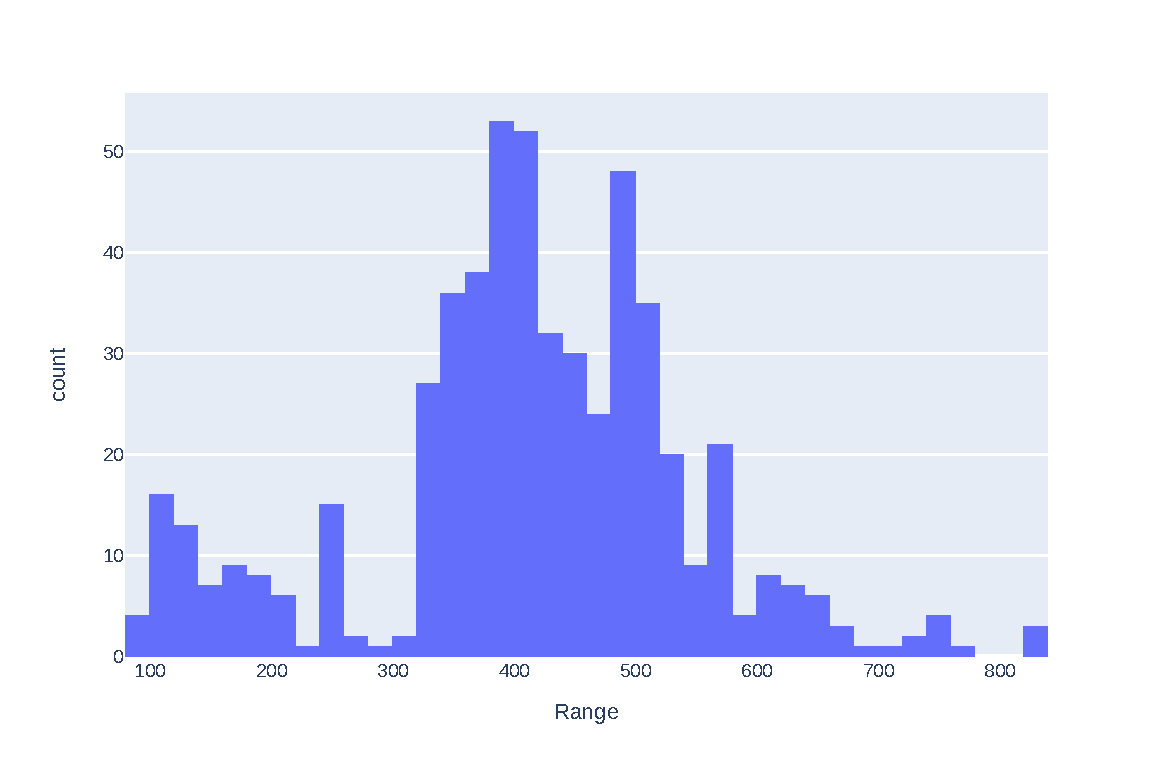
\includegraphics[width=\textwidth]{px.histogram.pdf}
\end{frame}

\begin{frame}[fragile]{Histogram with Summary Information}
Prepare some summary statistics:

\footnotesize
\begin{pythoncode}
# Calculating summary statistics
mean_v = fuel['Range'].mean()
median_v = fuel['Range'].median()
lower95 = fuel['Range'].quantile(0.025)
upper95 = fuel['Range'].quantile(0.975)

# Creating the density plot
fig = px.histogram(fuel, x='Range', 
         color_discrete_sequence=['pink'])
\end{pythoncode}
\end{frame}

\begin{frame}[fragile]{Histogram with Summary Information \small [cont'd]}
\footnotesize
\begin{pythoncode}
# Adding vertical lines and annotations
fig.add_vline(x=mean_v, line_dash='dash', 
      annotation_text=f'Mean = {round(mean_v)}', 
      annotation_position='top right')
fig.add_vline(x=median_v, line_dash='dot', 
      annotation_text=f'Median = {round(median_v)}', 
      annotation_position='bottom right')
fig.add_vline(x=lower95, line_dash='dot', 
      annotation_text=f'L95 = {round(lower95)}', 
      annotation_position='top left')
fig.add_vline(x=upper95, line_dash='dot', 
      annotation_text=f'U95 = {round(upper95)}', 
      annotation_position='bottom left')

fig.update_layout(
    title='Density Plot - Years 2012 to 2024',
    xaxis_title='Range (km)',
    yaxis_title='Proportion of Vehicles')
\end{pythoncode}
\end{frame}

\begin{frame}{Histogram with Summary Information}
    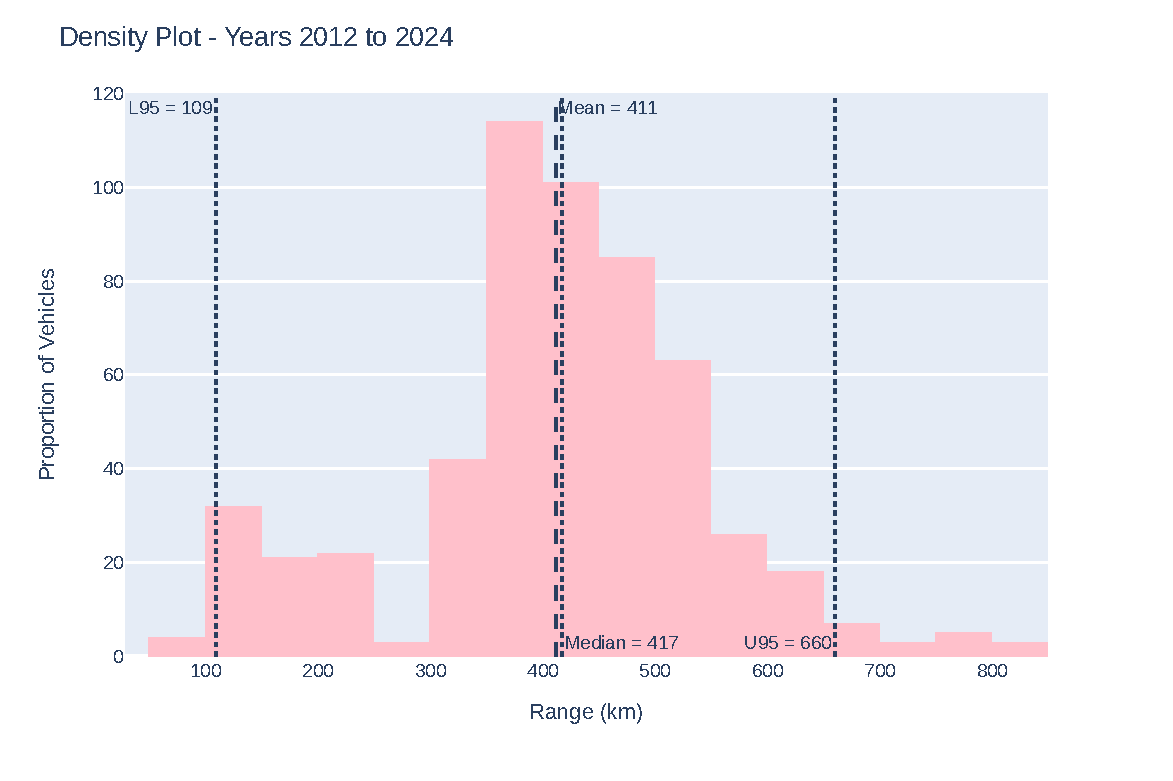
\includegraphics[width=\textwidth]{px.histogram2.pdf}
\end{frame}


\begin{frame}[fragile]{Column Chart}
\footnotesize
\begin{pythoncode}
fuel_grouped = fuel.groupby('Year').agg(
       meanCity=pd.NamedAgg('City', 'mean'),
       meanHwy=pd.NamedAgg('Hwy', 'mean')) \
         .reset_index()

fuel_long = pd.melt(fuel_grouped, 
                id_vars=['Year'], 
                value_vars=['meanCity', 'meanHwy'], 
                var_name='metric', 
                value_name='consumption')

fuel_long['metric'] = fuel_long['metric'] \
       .map({'meanCity': 'City', 
             'meanHwy': 'Highway'})
\end{pythoncode}
\end{frame}

\begin{frame}[fragile]{Column Chart \small [cont'd]}
Continued from previous slide ...
\footnotesize
\begin{pythoncode}
fig = px.bar(fuel_long, x='Year', y='consumption', 
   color='metric', barmode='group',
   labels={'consumption': 'Mean Cons\n(l/100km equiv)', 
           'metric': ''},
   title='Electric Vehicle Range (2012 to 2024)',
   color_discrete_map={'City': 'blue', 
                       'Highway': 'green'})

fig.update_layout(
    xaxis_title='Year', 
    yaxis_title='Mean Cons\n(l/100km equiv)')
\end{pythoncode}
\end{frame}

\begin{frame}{Column Chart}
  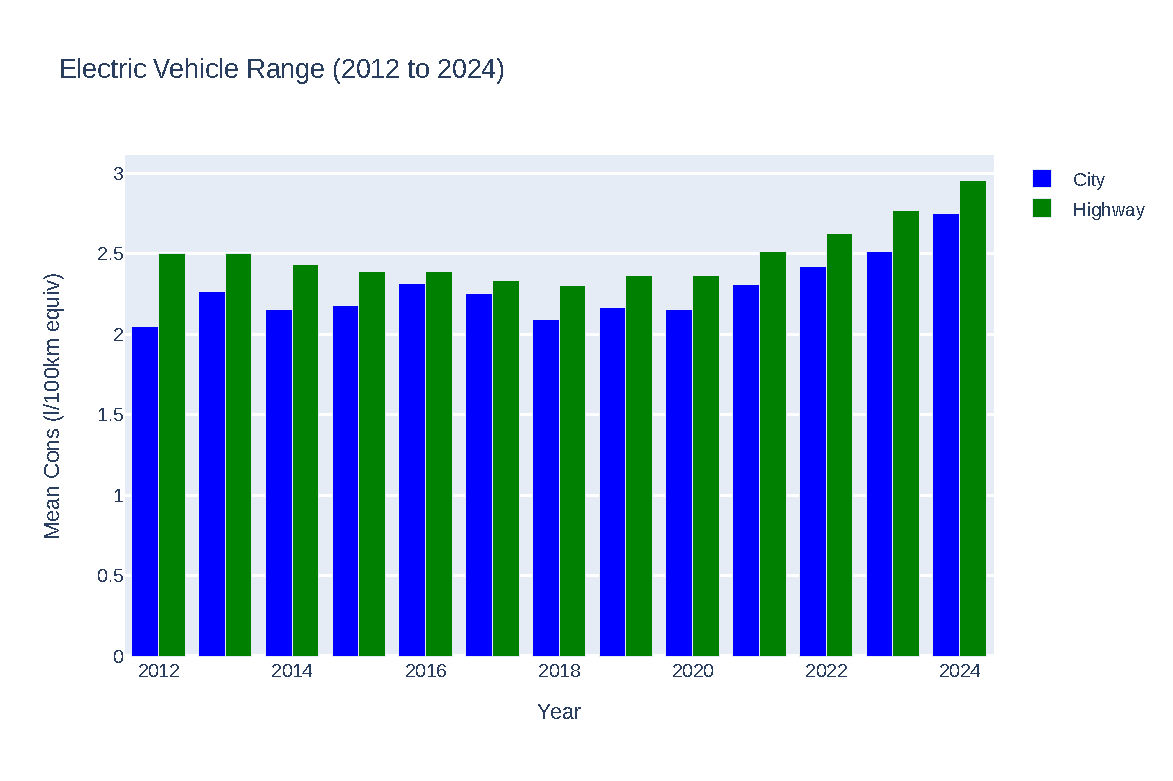
\includegraphics[width=\textwidth]{px.fuel.columns.pdf}
\end{frame}


\begin{frame}[fragile]{Column Chart (with Patterns)}
Prepare data
\footnotesize
\begin{pythoncode}
fig = px.bar(fuel_long, x='Year', y='consumption',
   pattern_shape = 'metric', barmode='group',
   pattern_shape_sequence \
       = ['.', 'x', '+', '|', '-', '/'],
   title = 'Electric Vehicle Range {2012 to 2024)',
   text_auto=True,
   template="simple_white",
   labels={'consumption': 'Mean Cons\n(l/100km equiv)', 
           'metric': ''})

fig.update_yaxes(tickformat=',.2r')
fig.update_traces(
      marker=dict(color='black', line_color='black', 
                  pattern_fillmode='replace'))
\end{pythoncode}
\end{frame}

\begin{frame}{Column Chart (with Patterns)}
  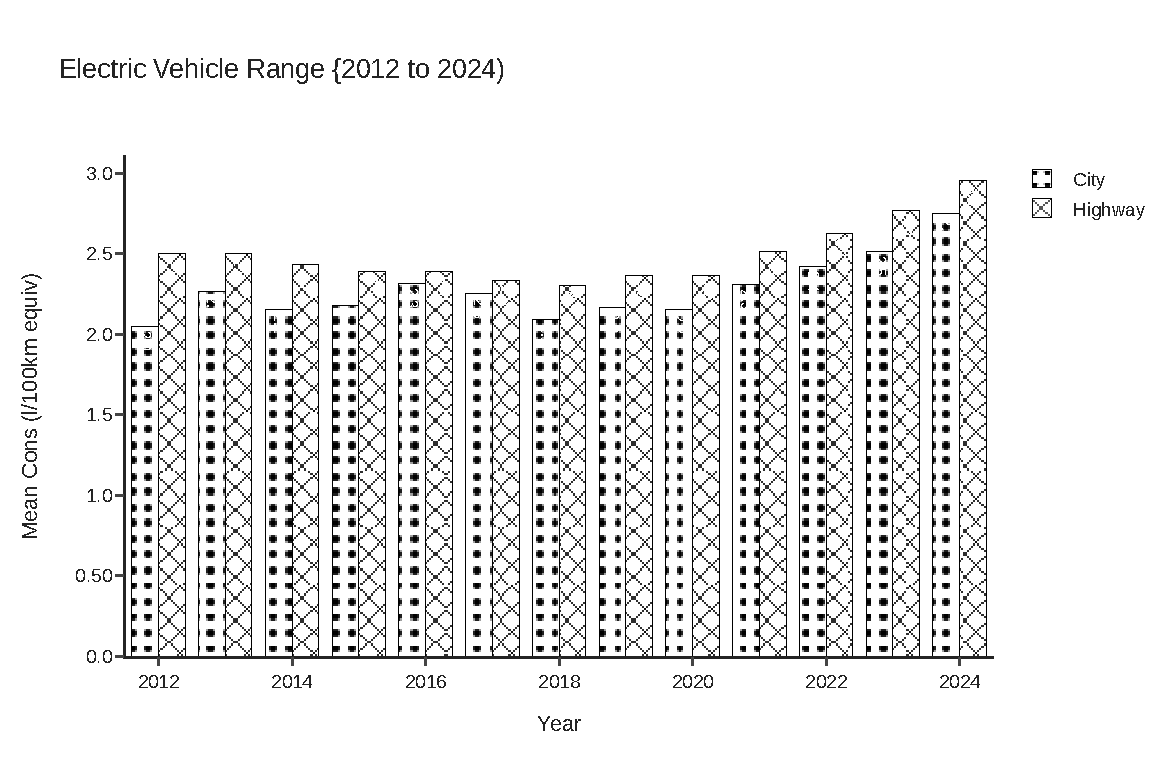
\includegraphics[width=\textwidth]{px.fuel.columnsPatterns.pdf}
\end{frame}


\begin{frame}[fragile]{Box Plot}
\footnotesize
\begin{pythoncode}
fuel_long = pd.melt(fuel, 
    id_vars=['Year'], value_vars=['City', 'Hwy'], 
    var_name='metric', value_name='consumption')

fig = px.box(fuel_long, 
         x=fuel_long['Year'].astype(str), 
         y='consumption', color='metric', 
         labels={'consumption': 'Mean Cons\n(l/100km)', 
                 'metric': ''},
         title='Electric Vehicles (2012 to 2024)')

fig.update_layout(
         xaxis_title='Year', 
         yaxis_title='Mean Cons\n(l/100km equiv)',
         legend_title_text='', 
         legend=dict(orientation="h", 
                     yanchor="top", y=1, 
                     xanchor="center", x=0.5))
\end{pythoncode}
\end{frame}

\begin{frame}{Box Plot}
  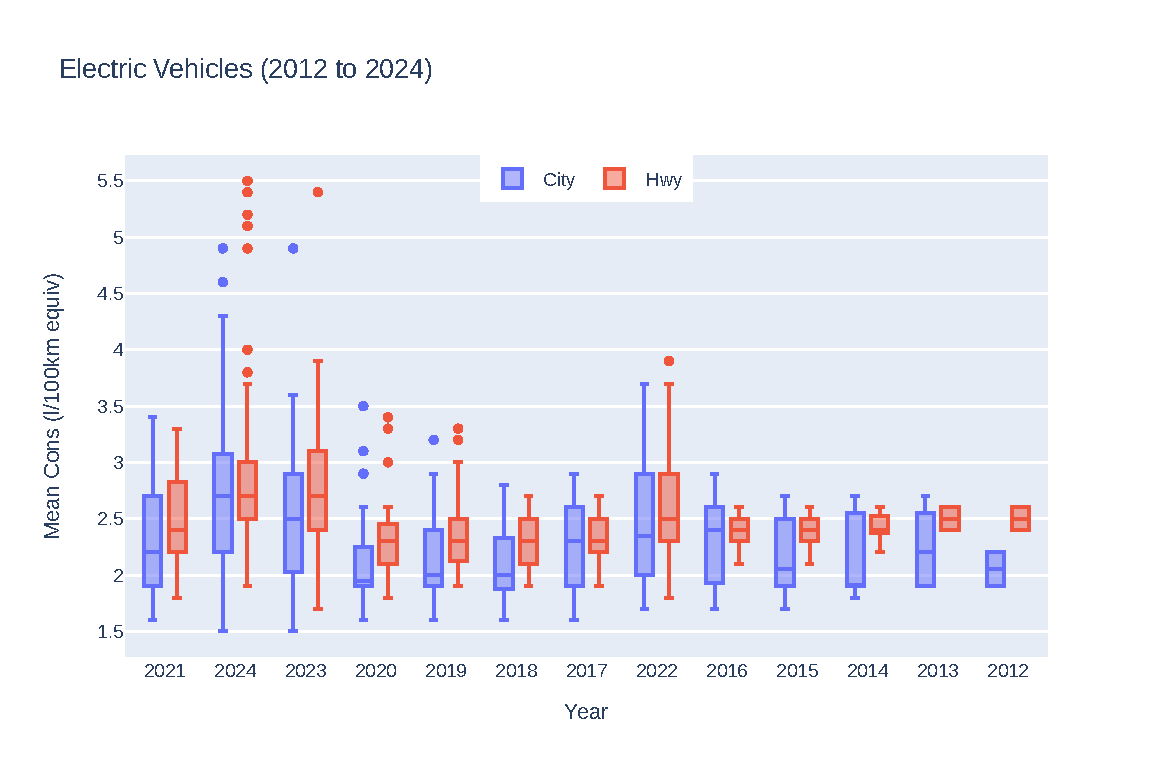
\includegraphics[width=\textwidth]{px.fuel.box.pdf}
\end{frame}

\begin{frame}[fragile]{Violin Plot}
\footnotesize
\begin{pythoncode}
fig = px.violin(fuel, 
       x=fuel['Year'].astype(str), 
       y='Comb', box=True, 
       points='all')

fig.update_traces(jitter=0.15, pointpos=0, 
       marker=dict(color='black', size=1, opacity=0.5))

fig.update_layout(xaxis_title='Year',
       yaxis_title='Mean Consumption\n(l/100km)',
       title='Electric Vehicle (2012 to 2024)',
       legend_title_text='')
\end{pythoncode}
\end{frame}

\begin{frame}{Violin Plot}
  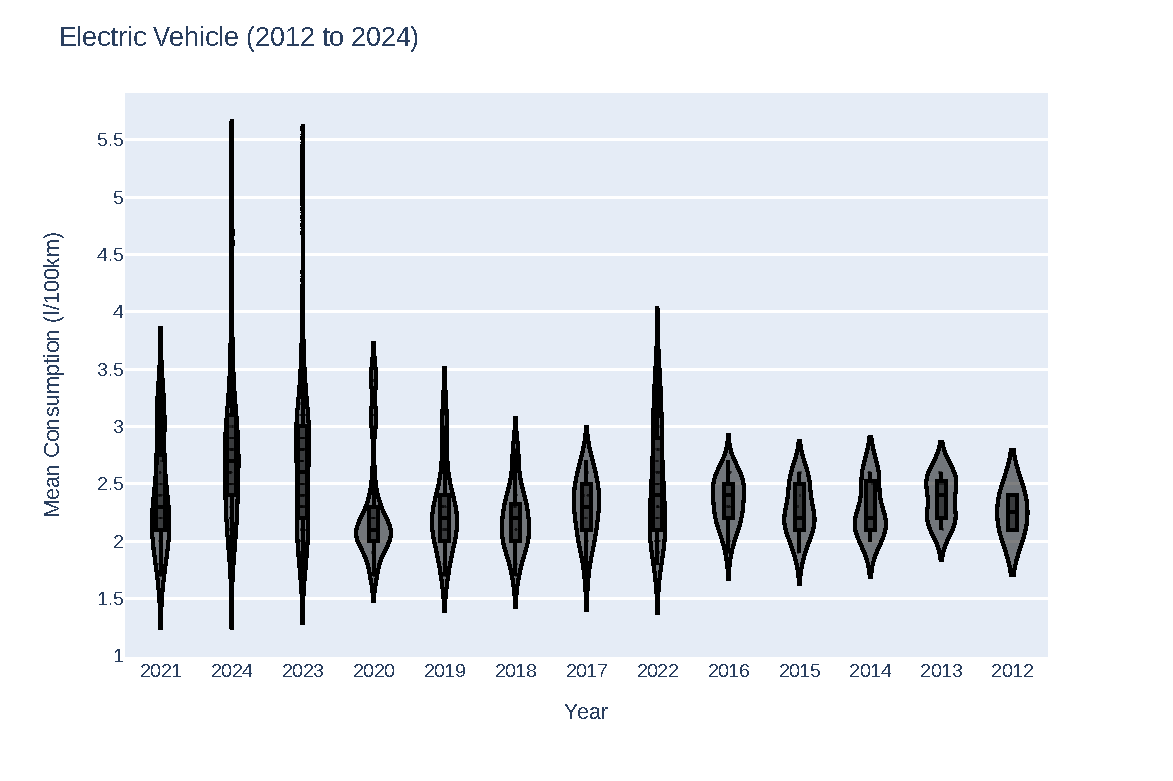
\includegraphics[width=\textwidth]{px.fuel.violin.pdf}
\end{frame}

\begin{frame}[fragile]{Count Plot}
\footnotesize
\begin{pythoncode}
count_df = fuel.groupby(['Year', 'Category']) \
   .size().reset_index(name='counts')

fig = px.scatter(count_df, 
   x='Year', y='Category', size='counts',
   color_discrete_sequence=['darkolivegreen'],
   labels={'Category': '', 
           'Year': 'Year', 
           'counts': 'Count'},
   title='EV Models by Category (2012 to 2024)')
\end{pythoncode}
\end{frame}

\begin{frame}{Count Plot}
  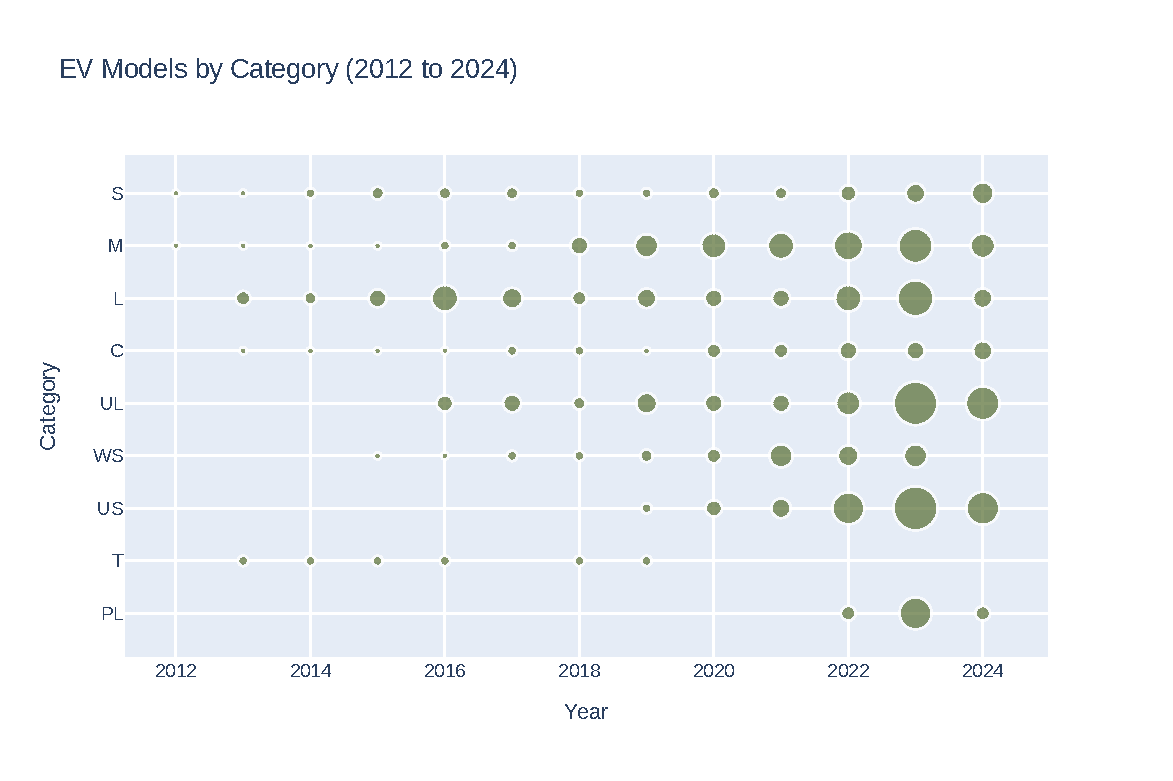
\includegraphics[width=\textwidth]{px.fuel.count.pdf}
\end{frame}

\begin{frame}[fragile]{Points Plot}
\footnotesize
\begin{pythoncode}
grouped_fuel = fuel.groupby(['Year', 'Category']).agg(
    totalcount=pd.NamedAgg('Range', 'size'),
    meanRange=pd.NamedAgg('Range', 'mean')
).reset_index()

fig = px.scatter(grouped_fuel, 
    x='Year', y='meanRange', size='totalcount', 
    color='Category', hover_name='Category', 
    labels={'meanRange': 'Range', 
            'totalcount': 'Number of Models'},
    title='EV by Year and Category (2012 to 2024)',
    size_max=20, opacity=0.8)

fig.update_layout(
    xaxis_title='Year',
    yaxis_title='Range',
    legend_title_text='Category',
    legend=dict(orientation="h", yanchor="bottom", 
                y=1.02, xanchor="right", x=1))
\end{pythoncode}
\end{frame}

\begin{frame}{Points Plot}
  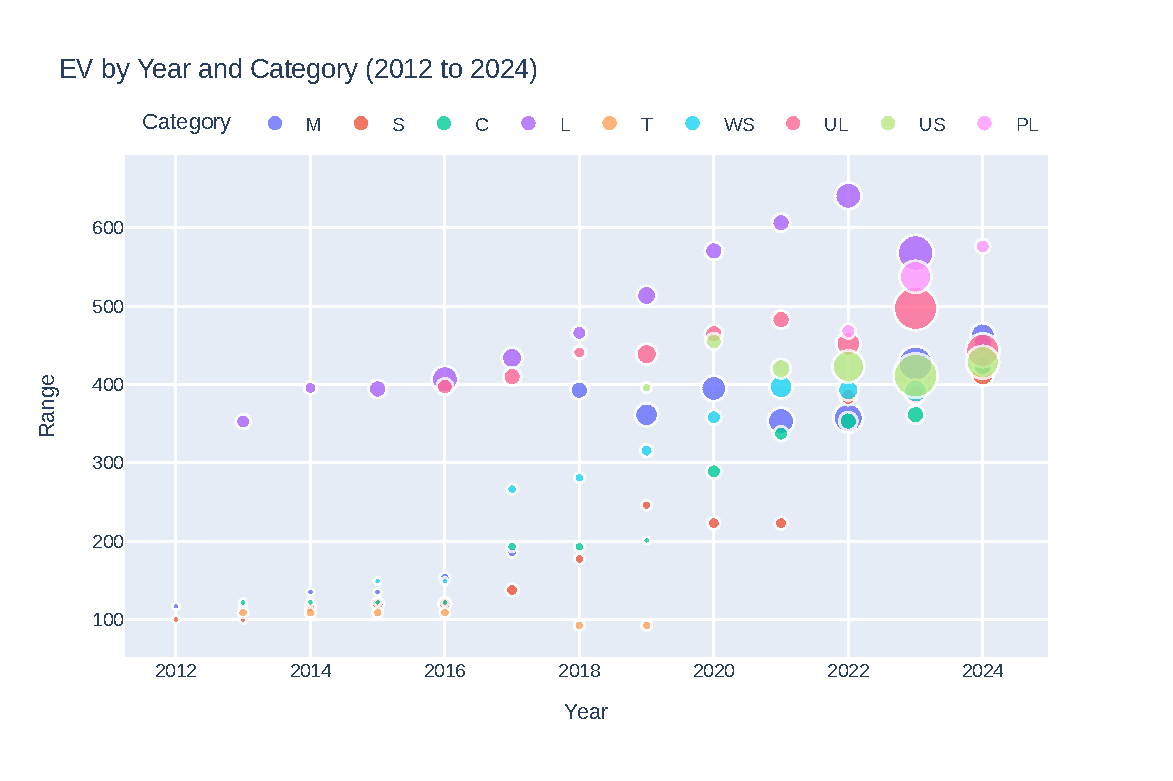
\includegraphics[width=\textwidth]{px.fuel.pointsSize.pdf}
\end{frame}

\begin{frame}[fragile]{Lines and Points Plot}
\footnotesize
\begin{pythoncode}
filtered_fuel = \
    fuel[(fuel['Year'] >= 2022) & 
         (fuel['Year'] <= 2023)]
filtered_fuel = \
    filtered_fuel[filtered_fuel['Comb'] <= 4]
filtered_fuel = \
    filtered_fuel[~filtered_fuel['Category'].isin(['PL', 'T'])]

fig = px.line(filtered_fuel, 
    x='Comb', y='Range', color='Category', 
    line_group='Category', markers=True, 
    labels={'Range': 'Range', 'Comb': 'Combined Fuel Consumption'},
    title='EV (2012 to 2024)')

fig.update_layout(
    xaxis_title='Combined Fuel Consumption',
    yaxis_title='Range',
    legend_title_text='Category',
    legend=dict(orientation="h", yanchor="bottom", 
                y=1.02, xanchor="right", x=1))
\end{pythoncode}
\end{frame}

\begin{frame}{Lines and Points Plot}
  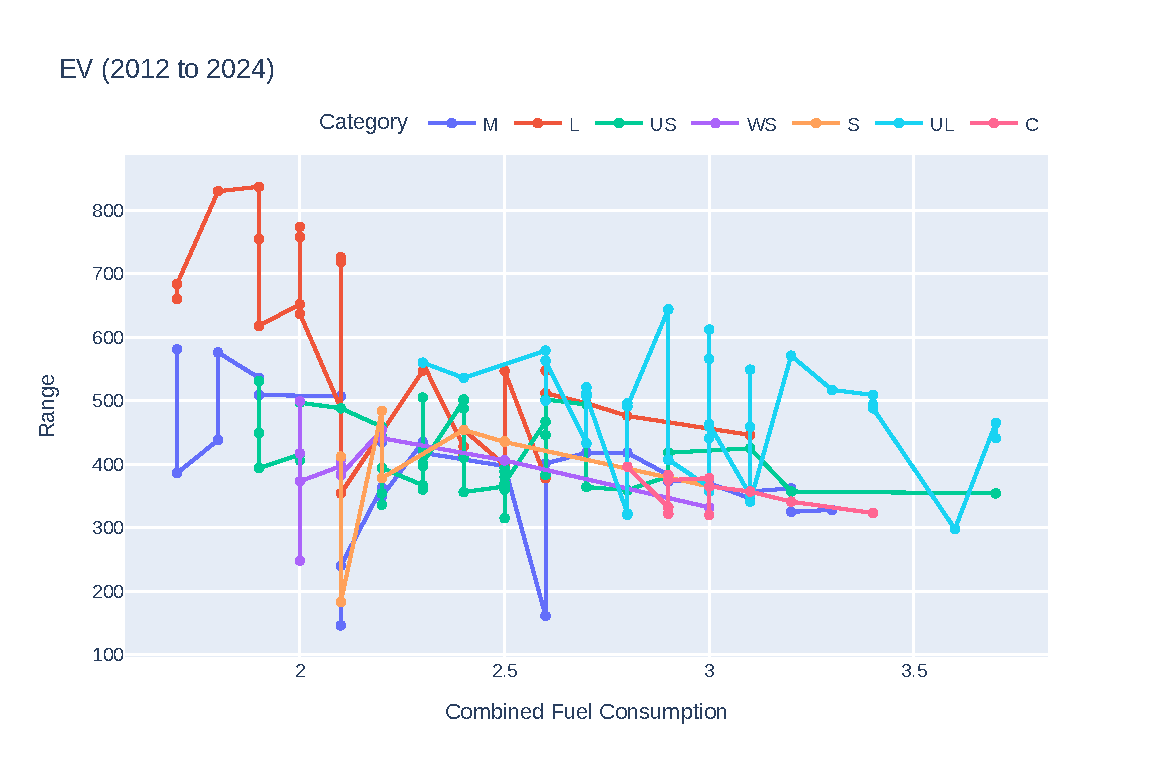
\includegraphics[width=\textwidth]{px.fuel.linesPoints.pdf}
\end{frame}


\begin{frame}[fragile]{Pie Chart}
\footnotesize
\begin{pythoncode}
fuel_2023 = \
    fuel[fuel['Year'] == 2023]
fuel_grouped = \
    fuel_2023.groupby('Make').size() \
    .reset_index(name='totalcount')
fuel_grouped = \
    fuel_grouped[fuel_grouped['totalcount'] >= 5]

fig = px.pie(fuel_grouped, 
    names='Make', values='totalcount', hole=0,
    title='EV Offerings by Make (2023, >= 5 models)',
    labels={'totalcount': 'Number of Models'})
\end{pythoncode}
\end{frame}

\begin{frame}[fragile]{Pie Chart \small [cont'd]}
Continued from previous slide \ldots
\footnotesize
\begin{pythoncode}
for i, row in fuel_grouped.iterrows():
    fig.add_annotation(text=str(row['totalcount']),
            x=row['Make'], y=row['totalcount'], 
            showarrow=False, font_color='lightgrey')

fig.update_layout(legend=dict(orientation="h", yanchor="bottom", 
    y=1.02, xanchor="right", x=1),
    showlegend=True, legend_title_text='Make')
\end{pythoncode}
\end{frame}

\begin{frame}{Pie Chart}
\centering
  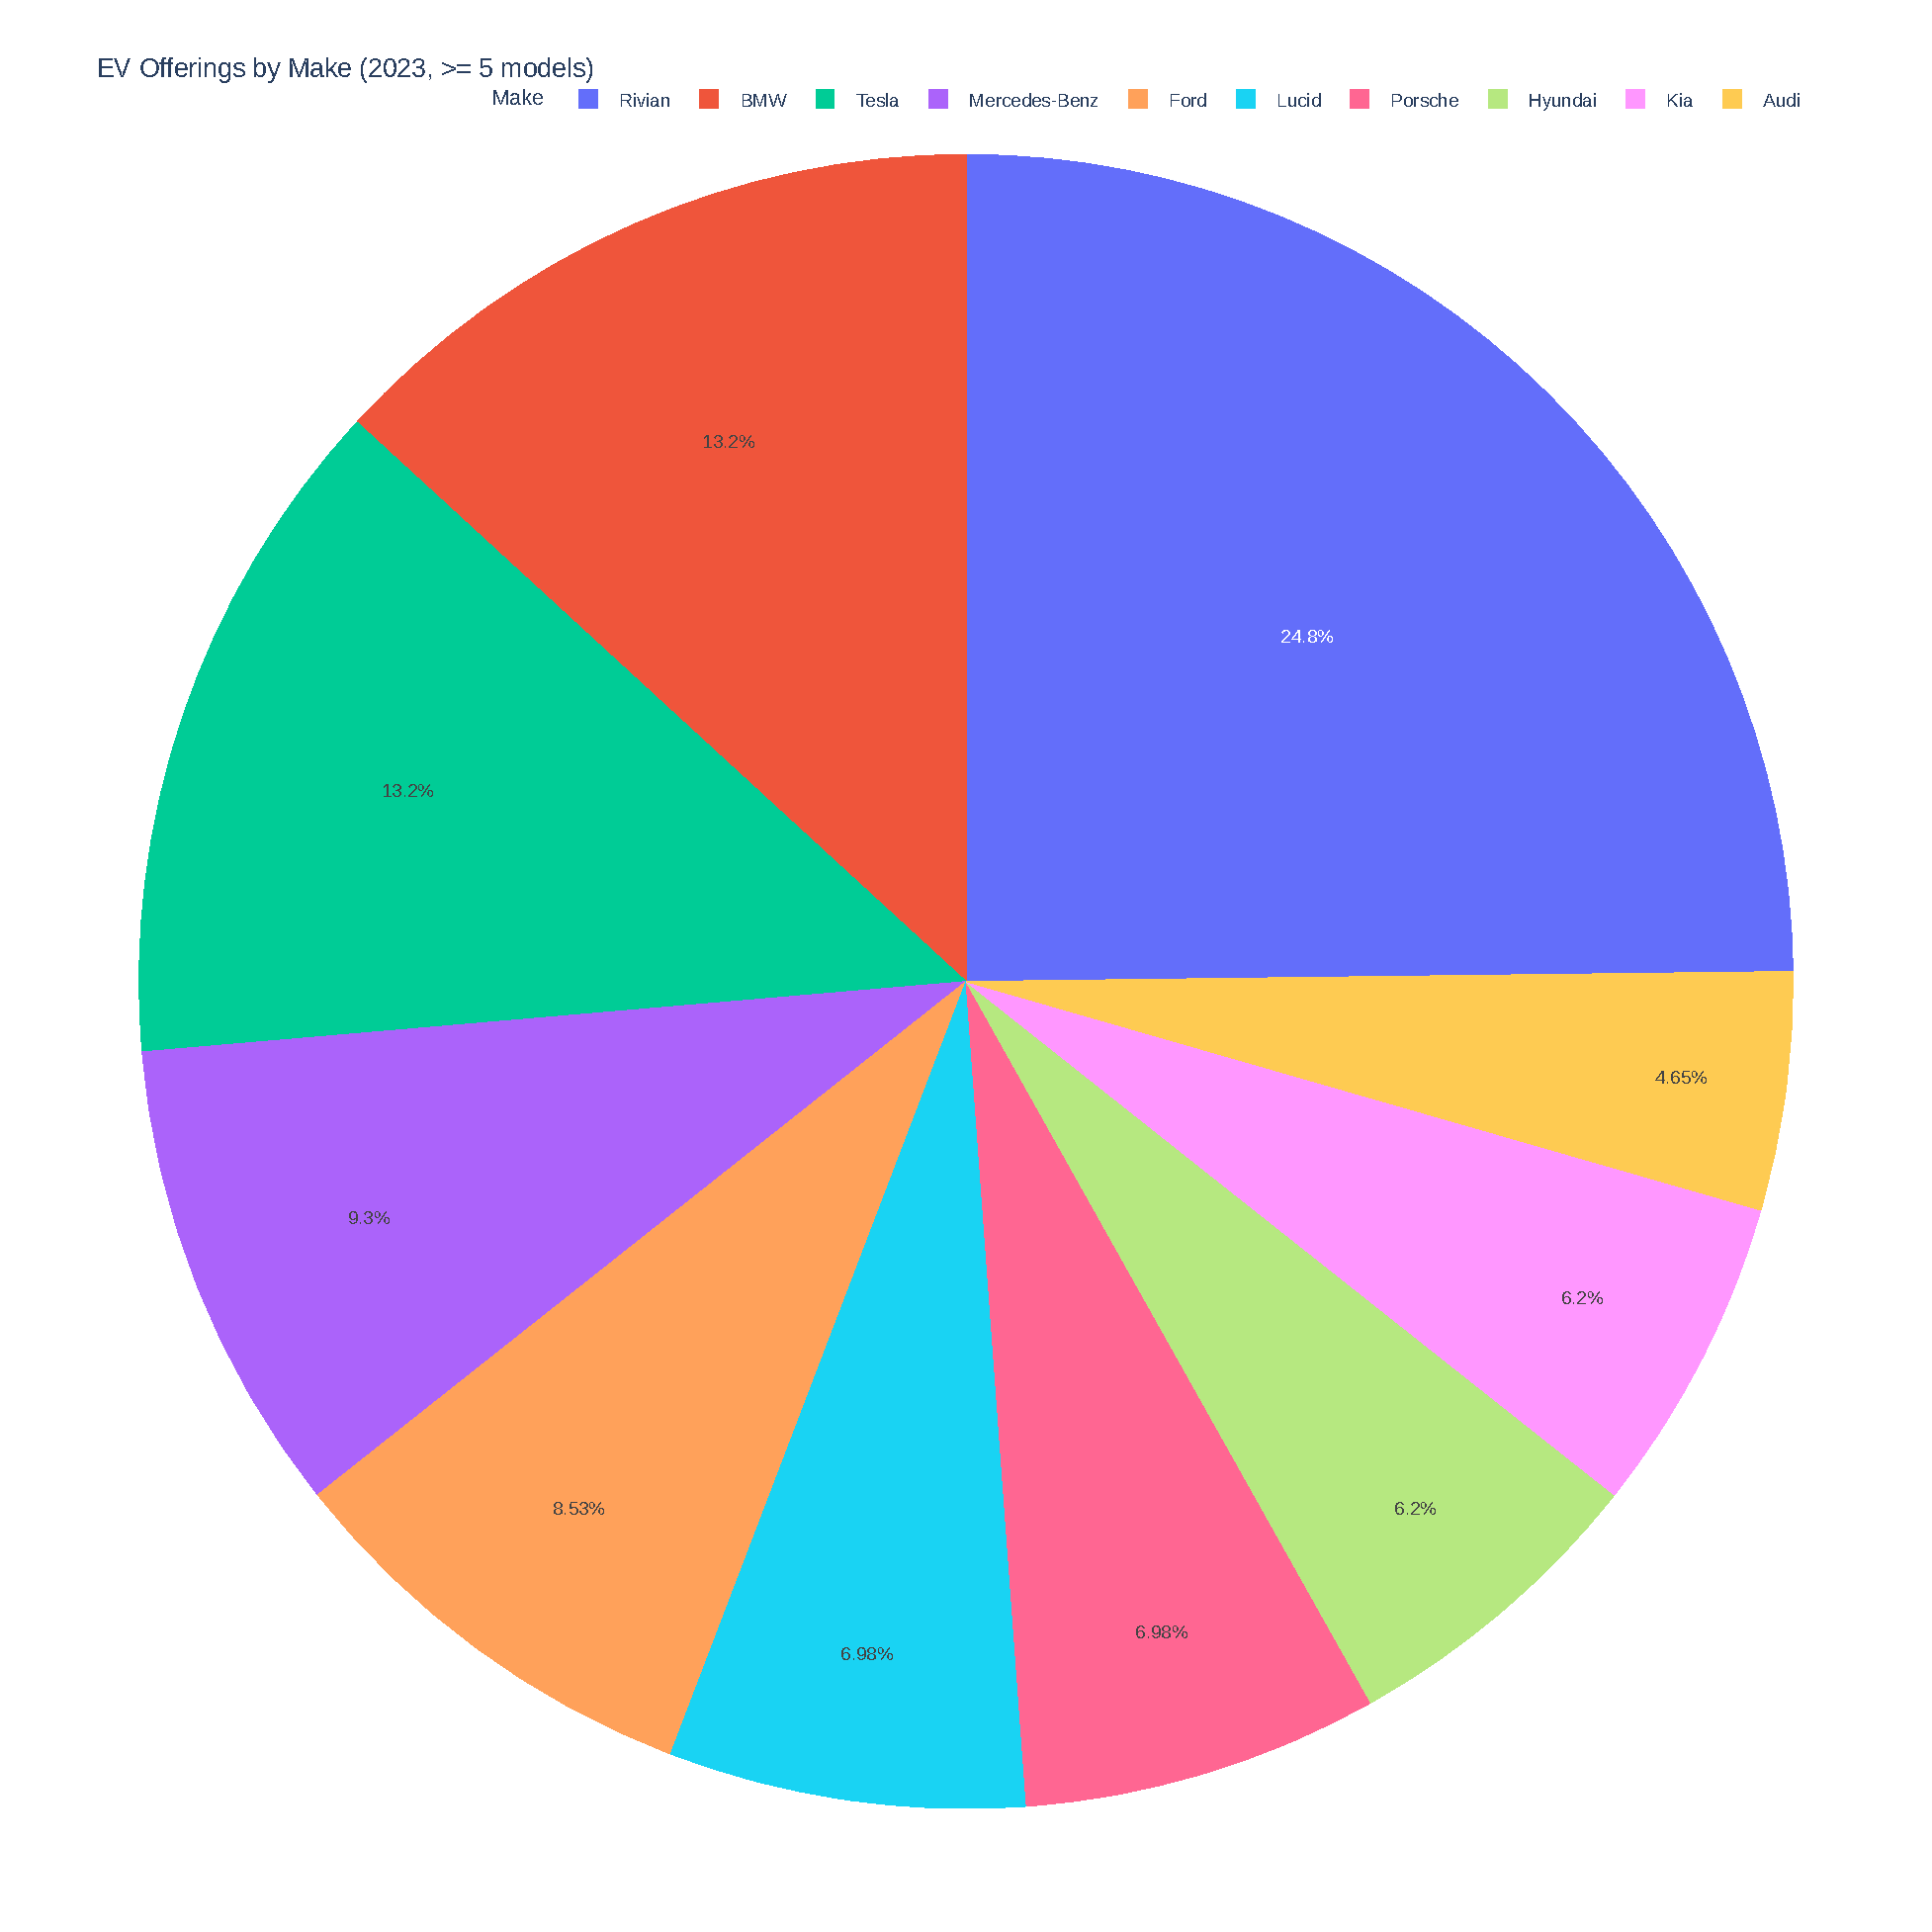
\includegraphics[width=.8\textwidth]{px.fuel.pie.pdf}
\end{frame}

\begin{frame}[fragile]{Donut Chart}
\footnotesize
\begin{pythoncode}
fig = px.pie(fuel_grouped, 
    names='Make', values='totalcount', hole=0.4,
    title='EV Offerings by Make (2023, >= 5 models)',
    labels={'totalcount': 'Number of Models'})
\end{pythoncode}
\end{frame}

\begin{frame}{Pie Chart}
\centering
  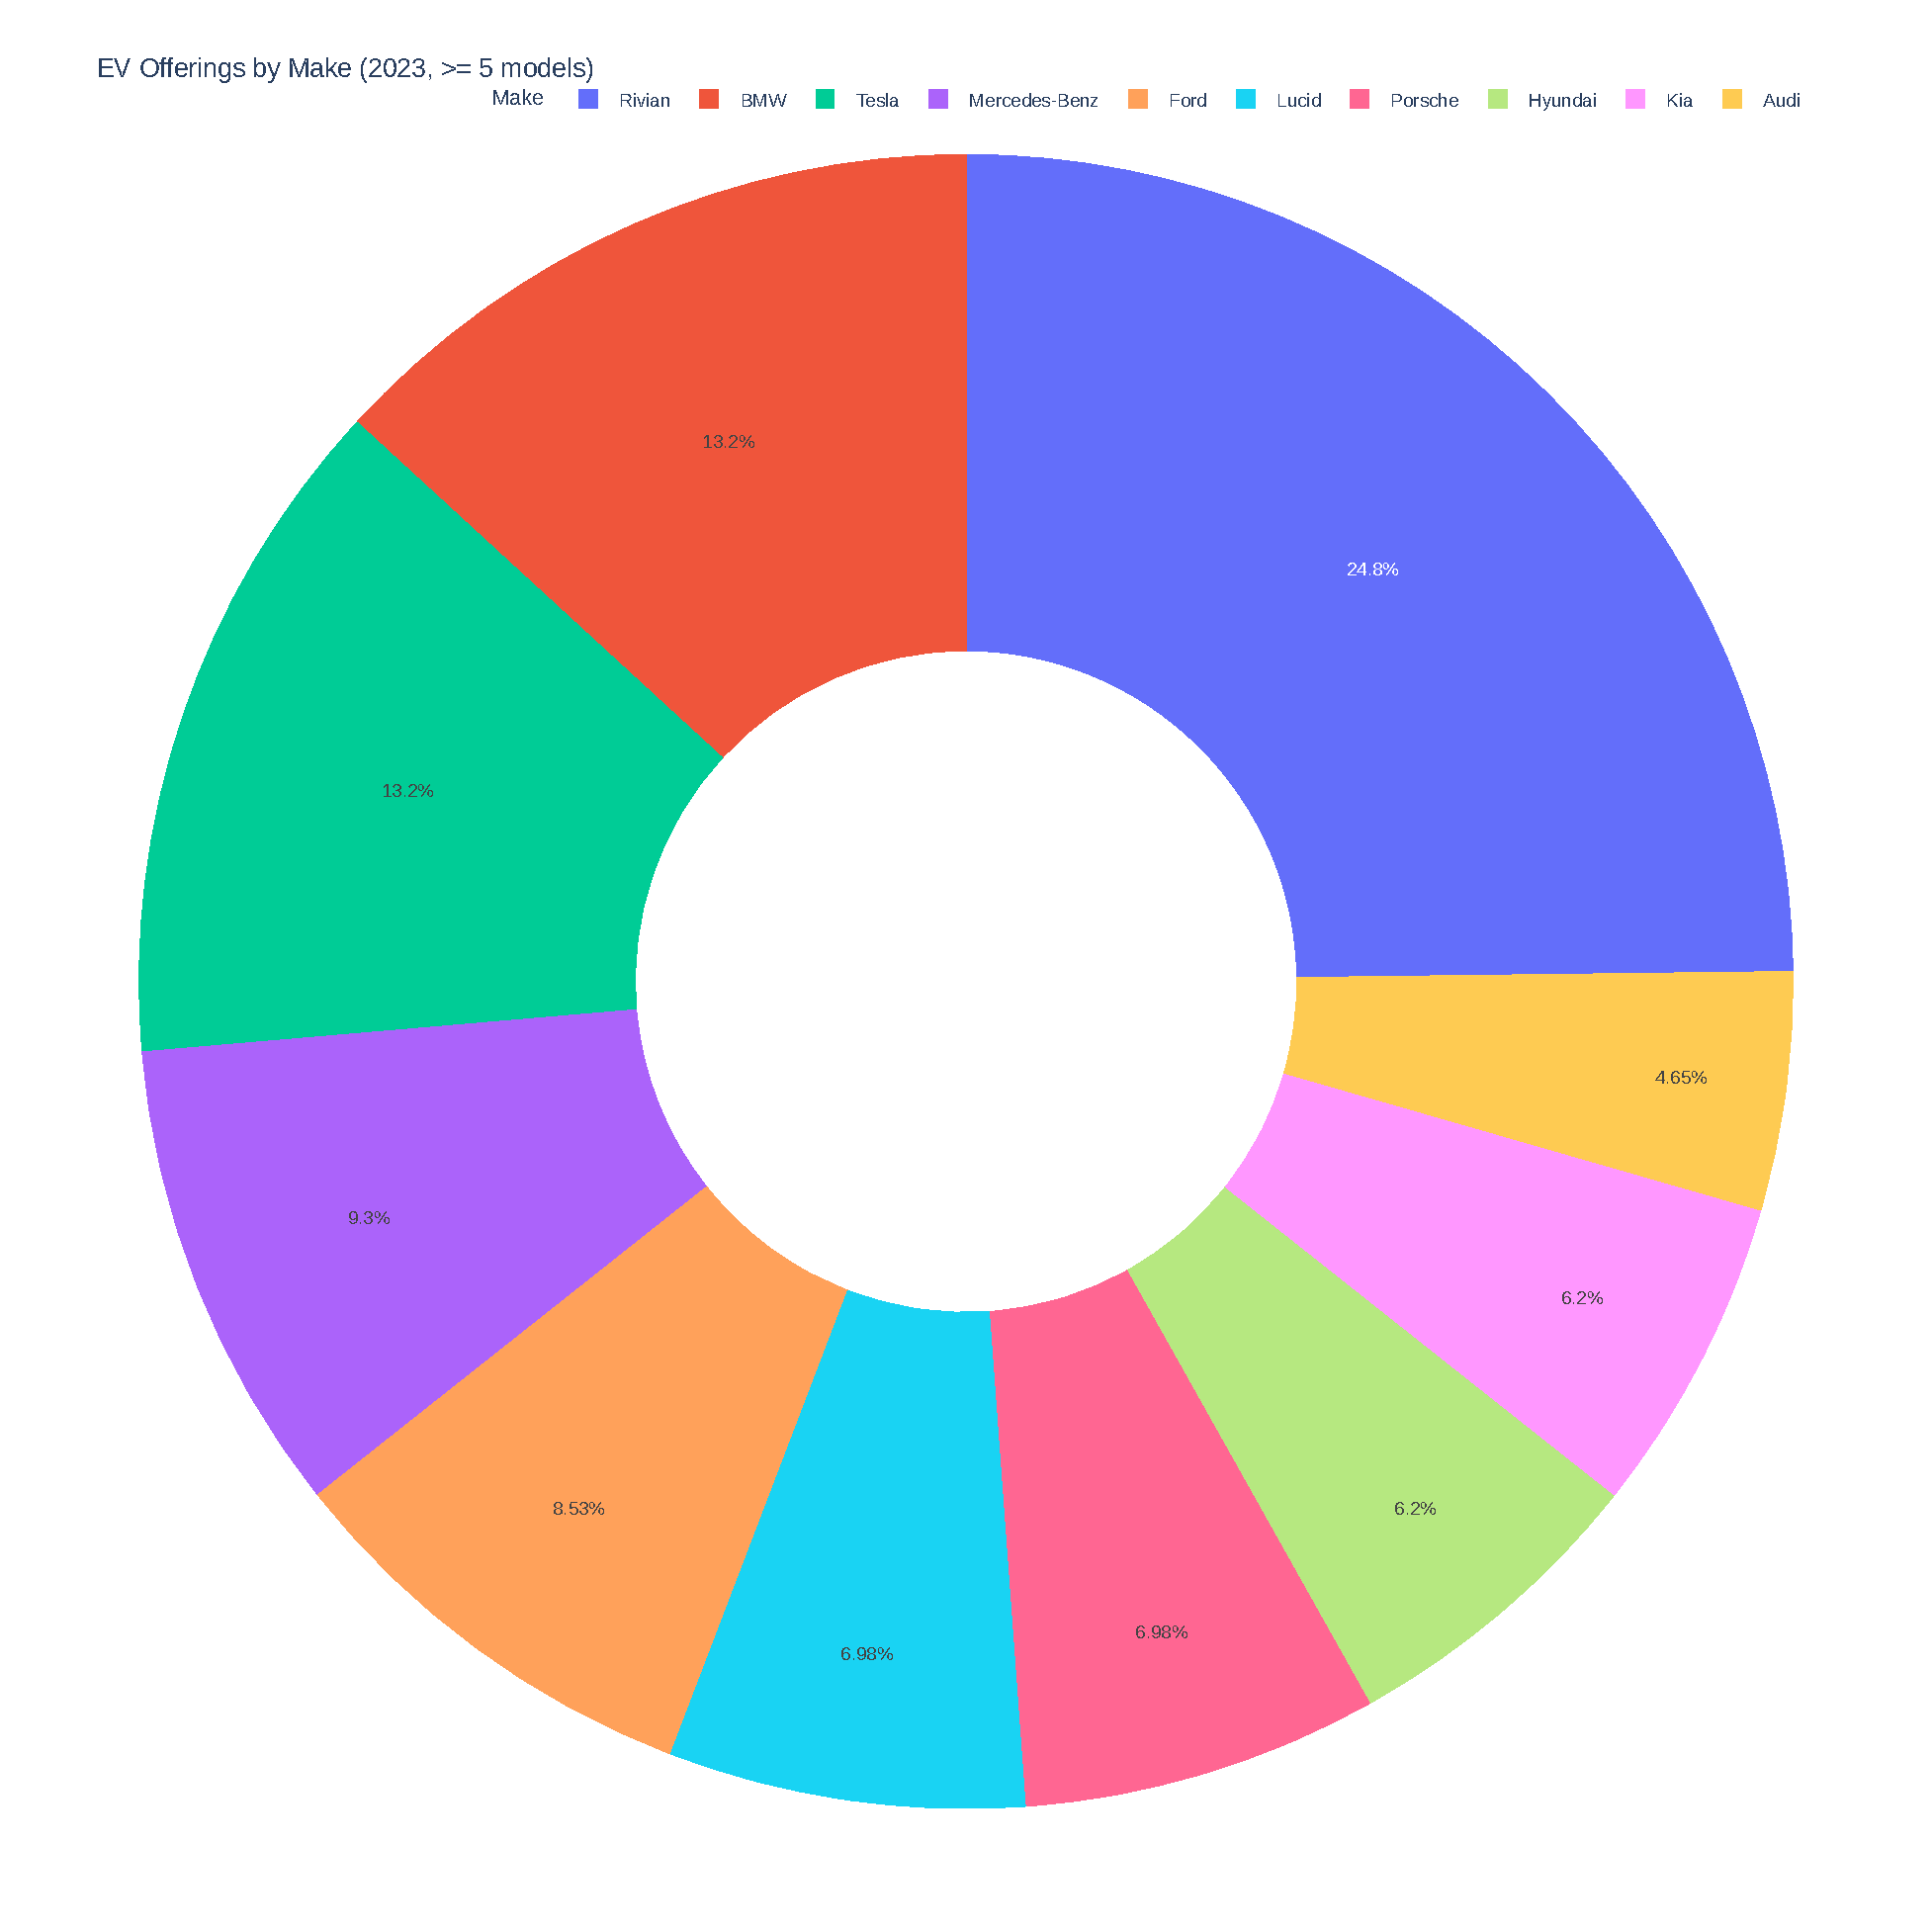
\includegraphics[width=.8\textwidth]{px.fuel.donut.pdf}
\end{frame}


\begin{frame}[fragile]{Radar Plot}
\footnotesize
\begin{pythoncode}
from sklearn.preprocessing import MinMaxScaler

fuel_2023 = fuel[fuel['Year'] == 2023]
grouped = fuel_2023.groupby('Make').agg(
    meanCity=pd.NamedAgg('City',lambda x: 1/x.mean()),
    meanHwy=pd.NamedAgg('Hwy',lambda x: 1/x.mean()),
    meanRange=pd.NamedAgg('Range',lambda x: x.mean()/100),
    nModels=pd.NamedAgg('Make','size')
)
grouped = grouped[grouped['nModels'] >= 5]

grouped[['meanCity', 'meanHwy', 'meanRange']] = \
   MinMaxScaler().fit_transform(
      grouped[['meanCity', 'meanHwy', 'meanRange']])

melted = grouped.reset_index().melt(
    id_vars='Make', 
     value_vars=['meanCity', 'meanHwy', 'meanRange'])
\end{pythoncode}
\end{frame}

\begin{frame}[fragile]{Radar Plot \small [cont'd]}
Continued from previous slide \ldots
\footnotesize
\begin{pythoncode}
fig = px.line_polar(melted, 
     r='value', 
     theta='variable', 
     color='Make', 
     line_close=True,
     labels={'variable': '', 
             'value': '', 
             'Make': 'Make'},
     title='EV Data (Makes with more than 5 models)')
\end{pythoncode}
\end{frame}

\begin{frame}{Radar Plot}
\centering
  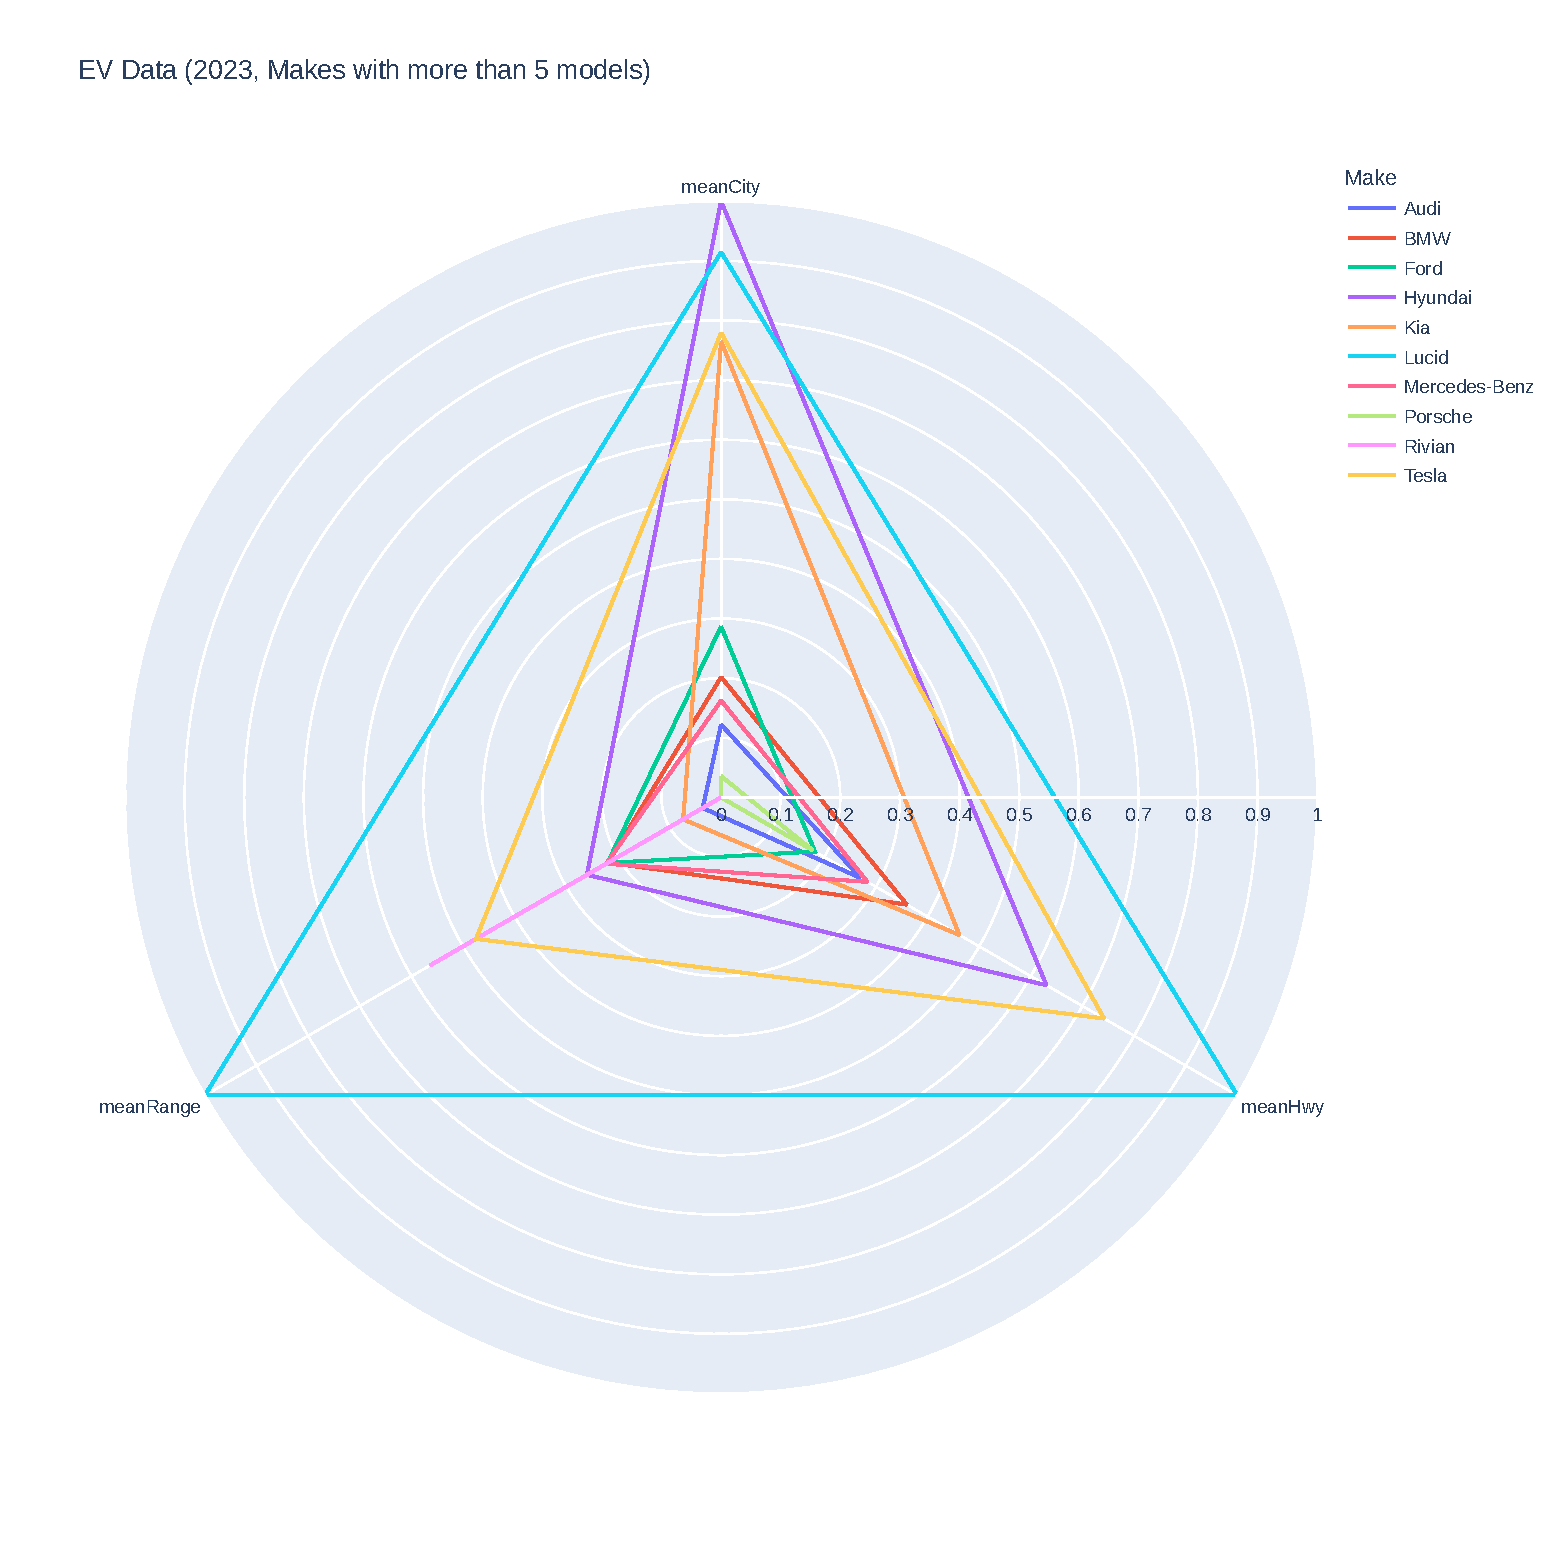
\includegraphics[width=.8\textwidth]{px.fuel.radar.pdf}
\end{frame}



\begin{frame}[fragile]{Local Regression Smoothing Plot}
\footnotesize
\begin{pythoncode}
fig = px.scatter(fuel, 
    x='Year', y='Range', trendline='lowess',
    labels={'Range': 'Mean Range (km)'},
    title='EV Range by Year')

fig.update_layout(xaxis_title='Year',
                  yaxis_title='Mean Range (km)')
\end{pythoncode}
\end{frame}

\begin{frame}{Local Regression Smoothing Plot}
  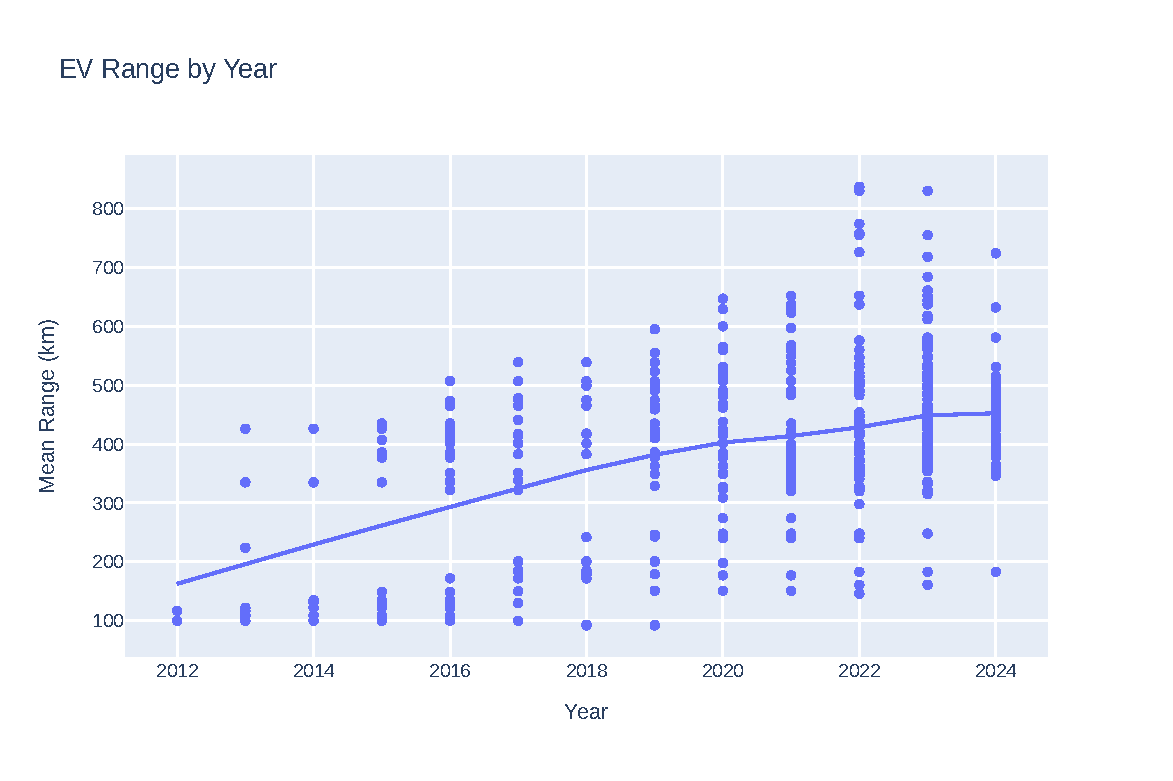
\includegraphics[width=\textwidth]{px.fuel.linesSmooth.pdf}
\end{frame}



\begin{frame}[fragile]{2D Density Plot}
\footnotesize
\begin{pythoncode}
import plotly.graph_objects as go

fig = px.scatter(fuel, 
    x='Hwy', y='City',
    title='Fuel Consumption (2012 to 2024)')

fig.add_trace(go.Histogram2dContour(
    x=fuel['Hwy'], y=fuel['City'], 
    colorscale='Earth'))

fig.update_layout(legend=dict(orientation="h", yanchor="bottom", 
                  y=1.02, xanchor="right", x=1),
                  showlegend=False, plot_bgcolor='white')
\end{pythoncode}
\end{frame}

\begin{frame}{2D Density Plot}
  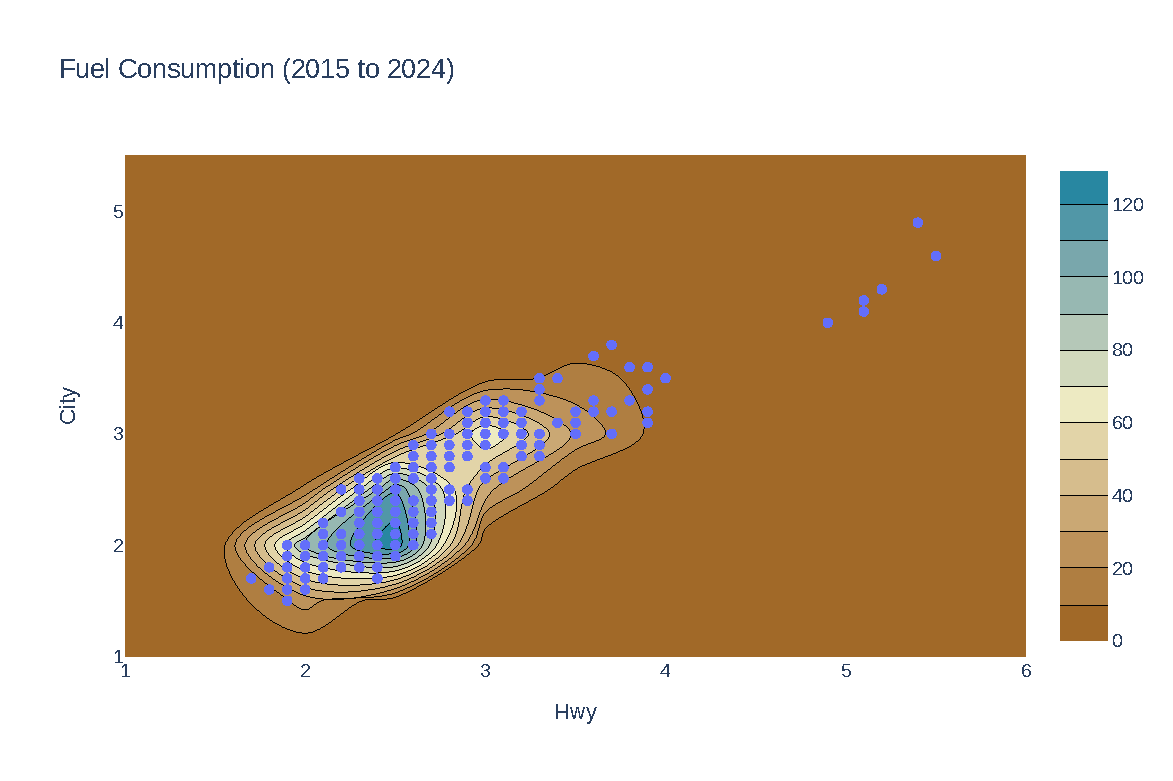
\includegraphics[width=\textwidth]{px.fuel.density2d.pdf}
\end{frame}

\begin{frame}[fragile]{Heatmap with Marginals}
\scriptsize
\begin{pythoncode}
fig = px.density_heatmap(fuel,
    x = 'City', y = 'Hwy',
    nbinsx=20, nbinsy=20,
    color_continuous_scale=px.colors.sequential.Viridis,
    marginal_x="histogram",
    marginal_y="histogram",
    title='EV Fuel Consumption Data',
    labels={"range" : "Range", 
           "Hwy": "Highway Economy", 
            "City": "City Economy"})
\end{pythoncode}
\end{frame}

\begin{frame}{Heatmap with Marginals}
  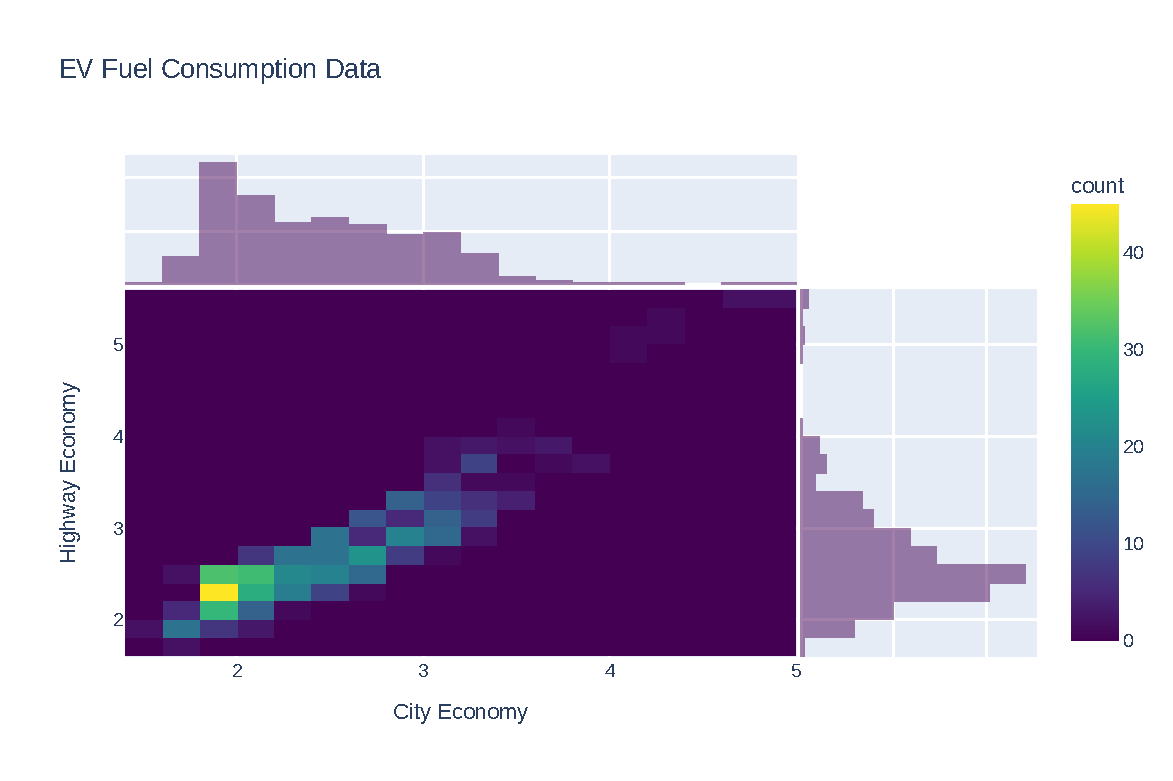
\includegraphics[width=\textwidth]{px.heatmap.pdf}
\end{frame}

\begin{frame}{Dashboards -- Live Demo}
\centering

  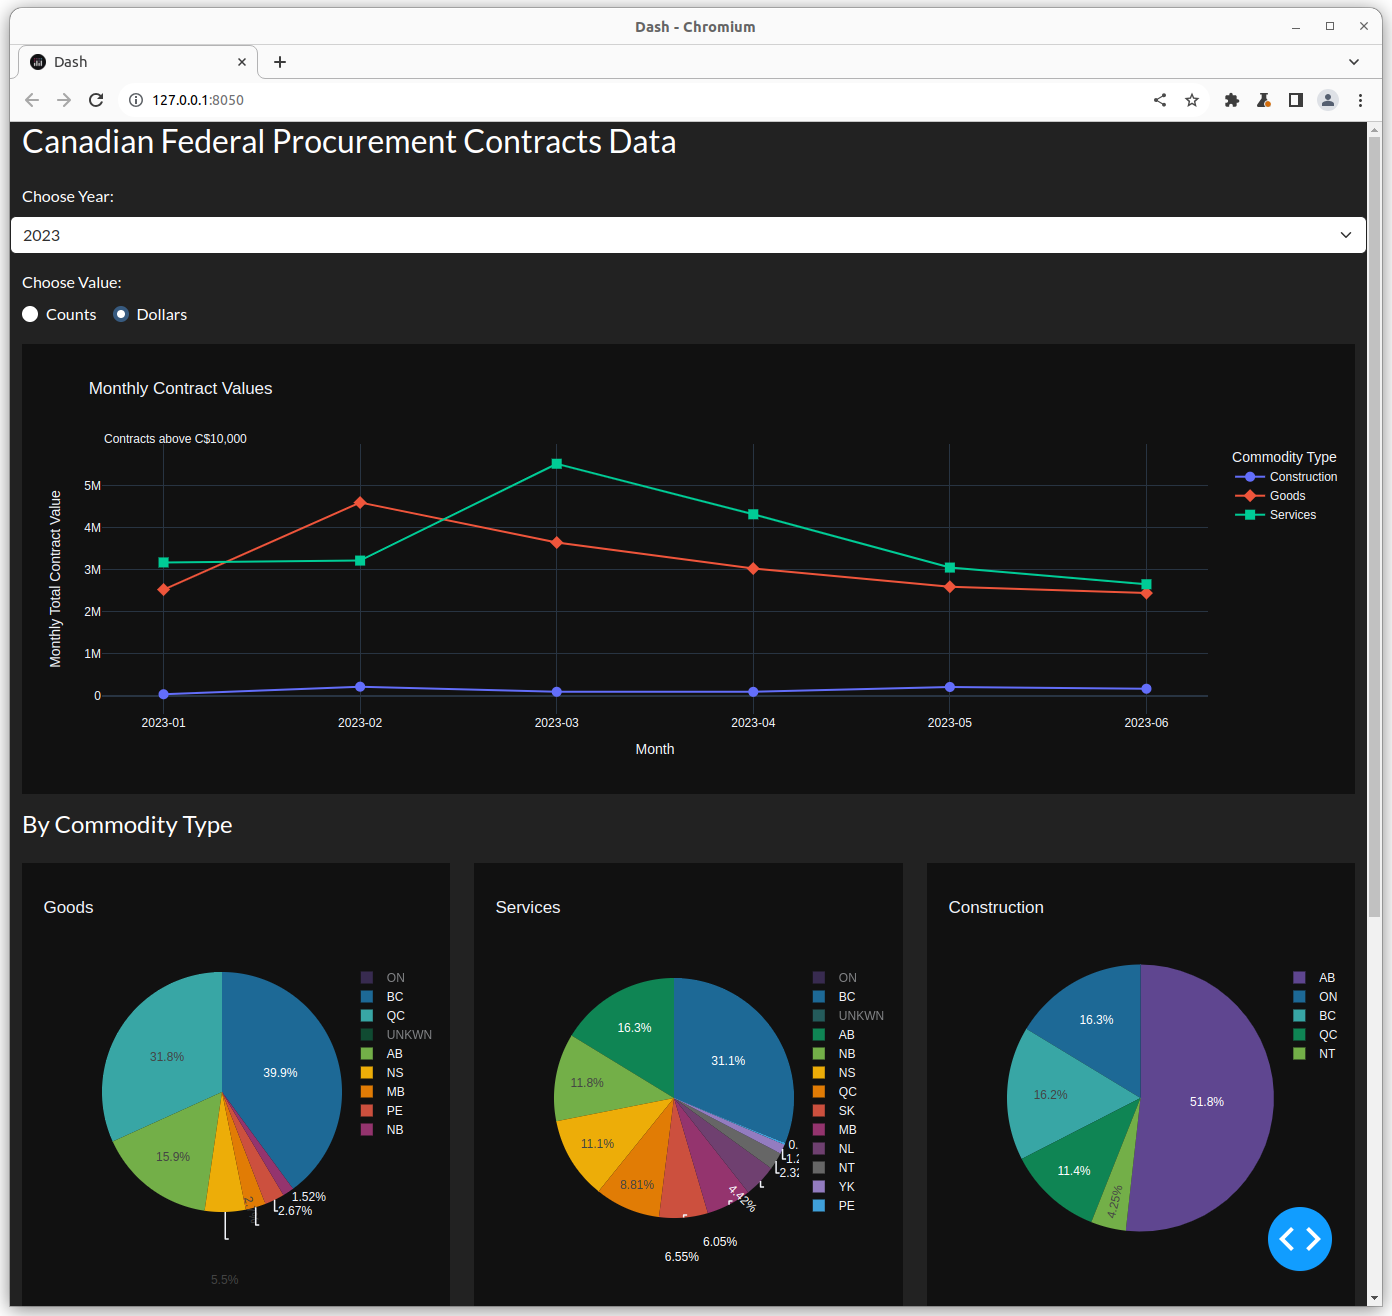
\includegraphics[width=.75\textwidth]{px.dash.screenshot.png}
\end{frame}

\begin{frame}{Hands-On Exercises}

\footnotesize
Using the Pagila database data from \url{https://evermann.ca/busi4720/rentals.csv}, create
\begin{enumerate}
   \item A histogram and/or density chart of film length by film category
   \item A column chart of the mean rental payments for films by film category
   \begin{itemize}
	  \footnotesize
      \item Add error bars to this chart
   \end{itemize}
   \item A scatter plot of total rental payments by year and week
   \begin{itemize}
	  \footnotesize
      \item Add a local regression line to this plot
   \end{itemize}
   \item A pie or donut chart of rental counts by film rating
\end{enumerate}
\textbf{Tips:}
\begin{itemize}
\item The Pandas \texttt{read\_csv()} function can read from a URL
\item The data is de-normalized, use the Pandas \texttt{drop\_duplicates()} function to get accurate film counts for exercise 1
\item Use \texttt{.dt.strftime('\%Y-\%W')} to extract the year and week from a datetime column in Pandas
\end{itemize}
\end{frame}


\end{document}
